





\subsection{Definition and Identification of `Pillar Tokens'}
\label{sec:pillar-identification}

To investigate this, we operationally categorize Rock Tokens based on their causal impact at inference time. \textbf{Pillar Tokens} are defined as those whose removal or perturbation degrades task accuracy, suggesting the model \emph{cannot reason without them}, while the remainder are deemed functionally neutral. 

\emph{\textbf{Intuition.}} The core idea is that if a token is truly load-bearing for reasoning, deleting it from the decoder should break the trajectory; if it only \emph{looks} ``hard'' due to high loss but lacks functional utility, its deletion should change nothing. We operationalize Pillarhood as exactly this causal, inference-time property. Given the post-OPD student $\pi_\theta$ and a candidate $v\in\widetilde{\mathcal{R}}$ (screening pool defined below), we form a knockout policy $\pi_\theta^{\setminus v}$ that sets the logit of $v$ to $-\infty$ at every decoding step and record the accuracy delta on a held-out benchmark $\mathcal{B}$:
\begin{equation}
\Delta_{\mathcal{B}}(v) = \mathrm{Acc}_{\mathcal{B}}\bigl(\pi_\theta^{\setminus v}\bigr) - \mathrm{Acc}_{\mathcal{B}}\bigl(\pi_\theta\bigr).
\label{eq:pillar-delta}
\end{equation}
A candidate $v$ is a \textbf{Strong Pillar} on $\mathcal{B}$ iff (i) $\Delta_\mathcal{B}(v)\le-\varepsilon$ ($\varepsilon=0.01$) and (ii) a paired bootstrap on per-problem indicators ($10{,}000$ resamples, $\alpha=0.05$) rejects $\mathrm{H}_0\!:\!\Delta=0$; symmetric thresholds at $+\varepsilon$ define Strong Stumbling Blocks, and all other candidates are Neutral. Accuracies are estimated by sampling at $T{=}1.0$ and averaging over independent rollouts to keep single-trajectory variance below the $\sim\!2\%$ effect scale.

The screening pool is a strict superset $\widetilde{\mathcal{R}}\supset\mathcal{R}$ of size $K_{\text{screen}}=200$ rather than the definitional $K=100$ set $\mathcal{R}$ of \S\ref{sec:rock_tokens}: $K=100$ is the stability/coverage sweet spot when $\mathcal{R}$ is treated as a vocabulary (qualitative analysis, gradient-zeroing in \S\ref{sec:rq3}), but Pillarhood is a per-token causal property and the bootstrap is a search for individual rare-but-real effects, so we trade selection stability below rank $100$ for a wider candidate pool. As a robustness check (Appendix~\ref{app:pillar_multiple_testing}), $6$ of the $10$ Strong Pillars --- including the strongest on each benchmark, ``\,certain'' on MATH-500 and ``-like'' on IFEval --- lie within the $K=100$ core. We probe the post-OPD student on two complementary benchmarks: MATH-500~\cite{lightman2023letsverifystepstep} for the trained reasoning capability and IFEval~\cite{zhou2023instruction} for instruction-following as an out-of-distribution control.


\subsection{Are Rock Tokens pillar? Experiments and findings}
\label{sec:pillar-experiments}

Table~\ref{tab:pillar-census} reports the full Pillar census from the bootstrap procedure across the $|\widetilde{\mathcal{R}}|=200$ screened candidates. The dominant feature of the per-token $\Delta_\mathcal{B}(v)$ distribution is not the tail but the centre: on both benchmarks the great majority of candidates fall inside the $\varepsilon$-band, indicating no detectable causal effect of their removal (visualization in Fig.~\ref{fig:pillar-delta-bar}, Appendix~\ref{app:pillar_multiple_testing}).

\begin{table}[t]
\centering
\caption{Pillar census over the $|\widetilde{\mathcal{R}}|=200$ screened Rock-Token candidates, by benchmark.}
\label{tab:pillar-census}
\begin{tabular}{lcccc}
\toprule
\textbf{Benchmark} & \textbf{Strong Pillar} & \textbf{Neutral} & \textbf{Strong Stumbling} & \textbf{Baseline acc.} \\
\midrule
MATH-500 & 7 (3.5\%)  & 193 (96.5\%) & 0 (0.0\%) & 0.750 \\
IFEval   & 3 (1.5\%)  & 197 (98.5\%) & 0 (0.0\%) & 0.752 \\
\midrule
\multicolumn{4}{l}{Cross-task agreement: 190 N$|$N, 7 P$|$N, 3 N$|$P, \textbf{0} P$|$P} & \\
\bottomrule
\end{tabular}
\end{table}

\paragraph{Multiple-testing considerations.} At $|\widetilde{\mathcal{R}}|=200$ candidates, $\sim\!10$ false rejections are expected by chance at $\alpha=0.05$, and neither Bonferroni nor Benjamini--Hochberg ($q\le 0.20$) retains any individual token (Appendix~\ref{app:pillar_multiple_testing}). We therefore read the per-token identifications above as exploratory \emph{candidate} Pillars. The population-level claim is carried by the \emph{sign} of the rejections: all $10$ fall on the Pillar (negative-$\Delta$) side and zero on the Stumbling side, a $10{:}0$ split with exact probability $2^{-10}\approx 0.002$ under the multiplicity-noise null --- a single global test that does not inflate with the number of candidates screened.

\medskip

Three observations follow. \textbf{First}, Pillars are rare: $3.5\%$ on MATH-500 and $1.5\%$ on IFEval --- the persistent high-KL criterion of \S\ref{ref:recalcitrant_tokens} over-selects causally relevant tokens by more than an order of magnitude. \textbf{Second}, Pillarhood is task-specific: no token is a Strong Pillar on both benchmarks (P$|$P$=0$ in Table~\ref{tab:pillar-census}), so the role of a token type depends on the task. \textbf{Third}, Strong Pillars are content-bearing tokens at decision points, not the structural delimiters that dominate the surface clustering of $\mathcal{R}$ in \S\ref{ref:recalcitrant_tokens}: MATH-500 examples include ``\,certain'', ``\,strategic'', ``\,Initialize'', ``\,programs'', ``Do''; IFEval includes ``\,tools'', ``\,trade'', ``-like''. The symmetric Strong-Stumbling direction is empty under inference-time knockout, an asymmetry we revisit at training time in \S\ref{sec:rq3}.


\subsection{Does Rock Token follow previous findings on `Forking Tokens'?}
\label{sec:pillar-vs-forking}

\emph{Intuition.} The dominant prior framing casts ``important tokens'' as high-entropy decision points where the policy splits between alternative reasoning continuations: forking tokens in RLVR~\cite{wangbeyond}, and the (entropy~$\cup$~student--teacher-divergence) taxonomy formalized for OPD by TIP~\cite{tip2026} and related token-reweighting work~\cite{yang2025token,wu2025mitigating}. If our Pillars were the inference-time projection of any of these training-time importance criteria, knockout $\Delta_\mathcal{B}(v)$ should be predicted by entropy, by KL, or by some combination thereof.

\begin{figure}[t]
  \centering
  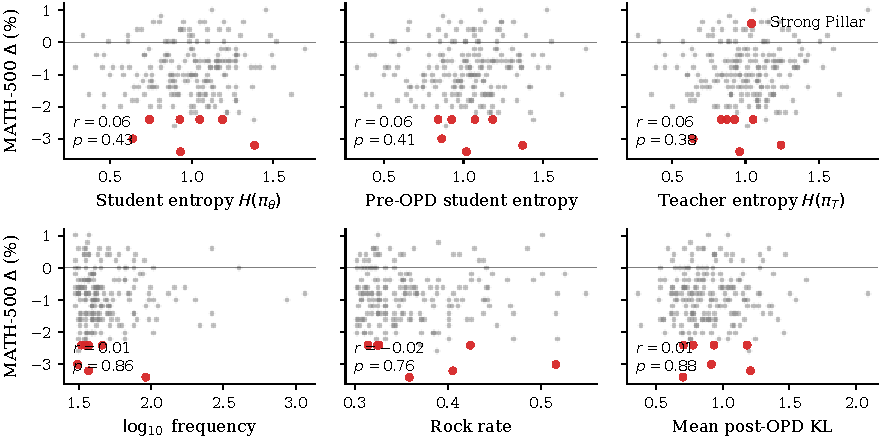
\includegraphics[width=\linewidth]{Figures/Section5/pillar_vs_predictors.pdf}
  \caption{\textbf{Pillarhood is not predicted by entropy, frequency, or
  loss.} MATH-500 knockout $\Delta$ for each of the $|\widetilde{\mathcal{R}}|=200$ screened candidates
  (Strong Pillars in red) plotted against six candidate predictors:
  post- and pre-OPD student entropy, teacher entropy, log-frequency, rock
  rate, and mean post-OPD KL. Annotated $r,p$ are Pearson correlations
  over all 200 candidates. None reach $|r|>0.07$.}
  \label{fig:pillar-vs-predictors}
\end{figure}

\emph{Findings.} Figure~\ref{fig:pillar-vs-predictors} scatters MATH-500 knockout $\Delta_{\mathrm{MATH500}}(v)$ against six candidate predictors --- pre/post-OPD student entropy, teacher entropy, $\log_{10}$ frequency, rock rate, and post-OPD KL --- and \emph{none} reaches $|r|>0.07$; the same conclusion holds on IFEval and on three additional loss-based predictors (Table~\ref{tab:pillar-correlations}, Appendix~\ref{app:pillar_correlations}). Pillars are scattered across the entire entropy range, not concentrated where forking tokens reside, and they are not the tokens with the largest residual KL --- the criterion that $\mathcal{R}$ itself maximizes. Pillarhood is therefore an \emph{orthogonal} cut: a causal, behaviour-defined property that the existing entropy- and divergence-based taxonomies fail to surface, with the immediate methodological corollary that any token-importance scheme keyed to those signals risks suppressing exactly the tokens the student cannot reason without.

\begin{takeaway}
\textcolor{tabblue}{\textbf{Take-away}}~
Pillar Tokens are not Forking Tokens. Their causal role at inference is
uncorrelated with student entropy, teacher entropy, frequency, or
post-OPD KL ($|r| < 0.07$ on MATH-500), placing them outside the
importance taxonomies of prior work~\cite{wangbeyond,tip2026}.
\end{takeaway}

